\documentclass[aspectratio=169,10pt]{beamer}

\usepackage[utf8]{inputenc}
\usepackage[T1]{fontenc}
\usepackage[brazil]{babel}
\usepackage{graphicx}
\usepackage{booktabs}
\usepackage{tabularx}
\usepackage{amsmath}
\usepackage{xcolor}
\usepackage{hyperref}

% ---------- Tema e paleta (tons de café) ----------
\usetheme{Madrid}
\usecolortheme{seahorse}

\definecolor{cafeEscuro}{HTML}{4E342E}
\definecolor{cafeMedio}{HTML}{795548}
\definecolor{folhaVerde}{HTML}{2E7D32}
\definecolor{destaque}{HTML}{BF360C}
\definecolor{fundoClaro}{HTML}{F5F0EB}

\setbeamercolor{structure}{fg=cafeEscuro}
\setbeamercolor{title}{fg=white, bg=cafeEscuro}
\setbeamercolor{frametitle}{fg=white, bg=cafeEscuro}
\setbeamercolor{block title}{fg=white, bg=folhaVerde}
\setbeamercolor{block body}{bg=fundoClaro}
\setbeamercolor{alerted text}{fg=destaque}
\setbeamerfont{frametitle}{series=\bfseries}

\setbeamertemplate{navigation symbols}{}
\setbeamertemplate{footline}{
  \leavevmode%
  \hbox{%
  \begin{beamercolorbox}[wd=.35\paperwidth,ht=2.5ex,dp=1ex,leftskip=.3cm,rightskip=.3cm]{author in head/foot}%
    \usebeamerfont{author in head/foot}Natalia Salete Rodrigues
  \end{beamercolorbox}%
  \begin{beamercolorbox}[wd=.5\paperwidth,ht=2.5ex,dp=1ex,leftskip=.3cm,rightskip=.3cm]{title in head/foot}%
    \usebeamerfont{title in head/foot}TCD Etapa 01 --- Aprendizado de Máquina / PPGEELT
  \end{beamercolorbox}%
  \begin{beamercolorbox}[wd=.15\paperwidth,ht=2.5ex,dp=1ex,leftskip=.3cm,rightskip=.3cm plus1fil]{date in head/foot}%
    \usebeamerfont{date in head/foot}\insertframenumber{} / \inserttotalframenumber
  \end{beamercolorbox}}%
  \vskip0pt%
}

% ---------- Título ----------
\title[Classificação de Doenças em Café]{Classificação Automatizada de Doenças em Folhas de Café Robusta em Condições Reais de Cultivo}
\subtitle{Etapa 01 --- Definição do Problema e Análise Exploratória do Dataset RoCoLe}
\author[Natalia Salete]{Natalia Salete Rodrigues \\ \small \texttt{natsalete@ufu.br}}
\institute[PPGEELT/UFU]{Programa de Pós-Graduação em Engenharia Elétrica (PPGEELT) \\ Universidade Federal de Uberlândia \\[6pt] \small \textit{Docente:} Prof\textsuperscript{a}. Dr\textsuperscript{a}. Danielli A. Lima}
\date{\small \today}

\begin{document}

% =============================================================
\begin{frame}[plain]
  \titlepage
\end{frame}

% =============================================================
\begin{frame}{Contexto na pós-graduação}
  \begin{columns}[T]
    \column{0.58\textwidth}
    \textbf{Quem sou eu}
    \begin{itemize}
      \item Mestranda no PPGEELT/UFU (ingresso 2026)
      \item Área: \textit{Processamento da Informação}
      \item Linha: \textit{Metodologias e Técnicas da Computação}
    \end{itemize}

    \vspace{0.6em}
    \textbf{Minha dissertação (24 meses)}
    \begin{itemize}
      \item \textit{Deep Learning} para diagnóstico de doenças em folhas de café em condições reais de cultivo
      \item Foco: arquitetura com módulos de atenção multi-escala adaptados
      \item Meta: superar 85\,\% de acurácia em classificação multiclasse no \textit{dataset} RoCoLe
    \end{itemize}

    \column{0.4\textwidth}
    \begin{block}{Este TCD}
      É a \textbf{Etapa 2} do meu cronograma de mestrado (Preparação e Análise Exploratória do \textit{Dataset}), antecipada dentro da disciplina.
    \end{block}
    \vspace{0.4em}
    \begin{alertblock}{Duplo ganho}
      Entrego a Etapa 01 do TCD \textbf{e} produzo material reutilizável na minha dissertação.
    \end{alertblock}
  \end{columns}
\end{frame}

% =============================================================
\begin{frame}{Motivação}
  \begin{columns}[T]
    \column{0.55\textwidth}
    \textbf{O problema econômico}
    \begin{itemize}
      \item Brasil: $\sim$37\,\% da produção mundial de café
      \item Doenças foliares podem comprometer até \alert{30\,\% da safra} se não tratadas a tempo
    \end{itemize}

    \vspace{0.6em}
    \textbf{O problema técnico}
    \begin{itemize}
      \item Diagnóstico visual manual é lento, subjetivo e exige especialista
      \item Modelos atuais de \textit{deep learning} são treinados em imagens de laboratório (fundo uniforme) --- \alert{não generalizam para o campo}
    \end{itemize}

    \column{0.4\textwidth}
    \begin{block}{Oportunidade}
      \textit{Dataset} RoCoLe traz imagens capturadas \textbf{diretamente no campo} --- fundo complexo, iluminação variada, oclusões.
    \end{block}
    \begin{block}{Referência a superar}
      Santos et al.\ (2023): \\
      Binária: \textbf{95,19\,\%} (ResNet) \\
      Multiclasse: \textbf{78,03\,\%}
    \end{block}
  \end{columns}
\end{frame}

% =============================================================
\begin{frame}{Questão de pesquisa}
  \vfill
  \begin{block}{}
    \centering
    \textit{É possível discriminar automaticamente entre folhas saudáveis e folhas afetadas por diferentes patologias foliares (ferrugem em quatro níveis de severidade e ácaro-vermelho) em imagens de café robusta capturadas em condições reais de cultivo, utilizando uma representação tabular compacta de cor, textura e qualidade de imagem, de modo a estabelecer uma \textbf{linha de base classificatória} para confronto futuro com \textit{deep learning}?}
  \end{block}
  \vspace{0.8em}
  \begin{itemize}
    \item \textbf{Tarefa binária:} saudável vs.\ doente
    \item \textbf{Tarefa multiclasse:} seis classes (1 saudável + 5 patológicas)
  \end{itemize}
  \vfill
\end{frame}

% =============================================================
\begin{frame}{Dataset RoCoLe}
  \begin{columns}[T]
    \column{0.55\textwidth}
    \textbf{Origem:} Mendeley Data, DOI 10.17632/c5yvn32dzg.2 \\
    \textbf{Autoria:} Parraga-Alava et al.\ (2019) \\[0.3em]
    \textbf{Conteúdo}
    \begin{itemize}
      \item 1.560 imagens \texttt{.jpg}
      \item 4 formatos de anotação (CSV, JSON, COCO, Pascal VOC) + XLSX de classes
      \item Capturadas \textit{in situ} em plantações de café robusta
    \end{itemize}

    \vspace{0.4em}
    \textbf{Rotulagem}
    \begin{itemize}
      \item \textbf{Binária:} \textit{healthy} vs.\ \textit{unhealthy}
      \item \textbf{Multiclasse:} \textit{healthy}, \textit{rust\_level\_\{1..4\}}, \textit{red\_spider\_mite}
    \end{itemize}

    \column{0.42\textwidth}
    \begin{block}{Desafios do \textit{dataset}}
      \begin{itemize}
        \item Fundos complexos (solo, galhos, outras folhas)
        \item Variação de iluminação natural
        \item Múltiplos dispositivos de captura
        \item Oclusões parciais
      \end{itemize}
    \end{block}
  \end{columns}
\end{frame}

% =============================================================
\begin{frame}{Pipeline de preparação: de imagem a tabela}
  \begin{columns}[T]
    \column{0.42\textwidth}
    \textbf{Por que tabular?}
    \begin{itemize}
      \item Escolhi o \textbf{KNIME} como ferramenta por reunir, em um só ambiente, tudo que o TCD pede (classificação, avaliação e visualização)
      \item Quero uma \textbf{linha de base} clássica para confrontar depois com o \textit{deep learning} da dissertação
    \end{itemize}

    \vspace{0.4em}
    \textbf{Saída}
    \begin{itemize}
      \item \texttt{rocole\_features.csv}
      \item 1.560 linhas $\times$ 26 \textit{features} + 2 rótulos
    \end{itemize}

    \column{0.56\textwidth}
    \textbf{Grupos de \textit{features} extraídas}
    \vspace{0.3em}

    \footnotesize
    \renewcommand{\arraystretch}{1.2}
    \begin{tabularx}{\linewidth}{@{}Xc@{}}
      \toprule
      \textbf{Grupo} & \textbf{\#} \\
      \midrule
      Estatísticas de cor RGB & 6 \\
      Estatísticas de cor HSV & 6 \\
      Proporções cromáticas (saudável, ferrugem, necrose) & 3 \\
      Textura GLCM (Haralick) & 6 \\
      Dimensões da imagem & 3 \\
      Qualidade (brilho, Laplaciano) & 2 \\
      \midrule
      \textbf{Total} & \textbf{26} \\
      \bottomrule
    \end{tabularx}
  \end{columns}
\end{frame}

% =============================================================
\section{Insights da AED}

\begin{frame}{Insight 1 --- Desbalanceamento multiclasse severo}
  \begin{columns}[c]
    \column{0.55\textwidth}
    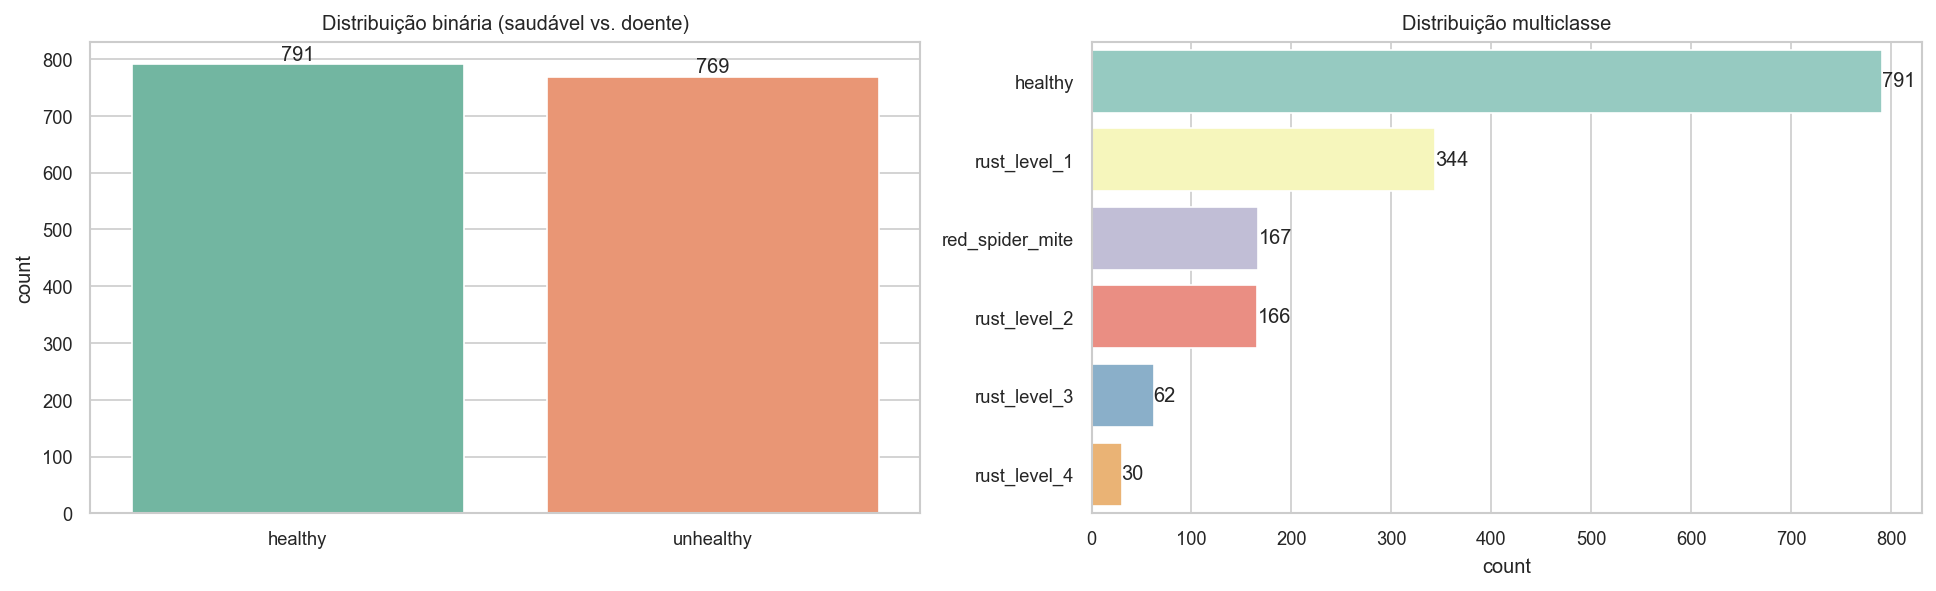
\includegraphics[width=\textwidth]{class_distribution.png}

    \column{0.45\textwidth}
    \begin{itemize}
      \item \textbf{Binária:} quase balanceado (791 vs.\ 769)
      \item \textbf{Multiclasse:} razão \alert{26,4$\times$} entre a maior e a menor classe
      \item Classes de ferrugem com decaimento monotônico: 344, 166, 62, \alert{30}
    \end{itemize}
    \vspace{0.5em}
    \begin{block}{Implicação}
      Explica a queda de 95\,\% $\to$ 78\,\% reportada por Santos et al.\ na transição binária $\to$ multiclasse.
    \end{block}
  \end{columns}
\end{frame}

% =============================================================
\begin{frame}{Insight 2 --- Variabilidade real de aquisição}
  \begin{center}
    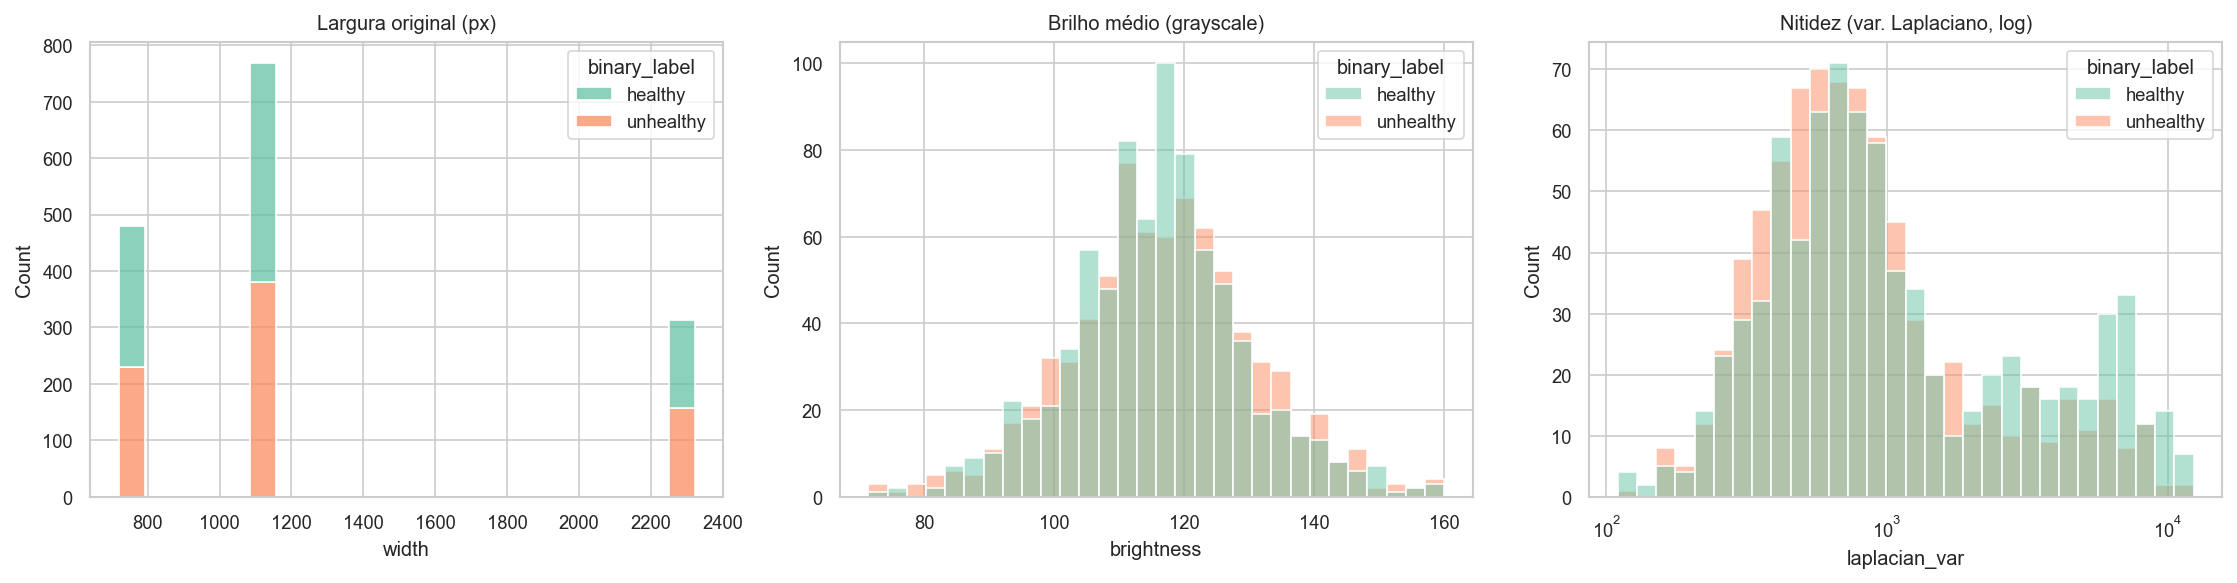
\includegraphics[width=0.92\textwidth]{image_quality.png}
  \end{center}
  \vspace{-0.3em}
  \begin{itemize}
    \item Resoluções de \textbf{$720{\times}1280$} a \textbf{$2322{\times}4128$} \textit{pixels}
    \item Brilho médio: $\mu=116{,}3$, $\sigma=13{,}9$
    \item Nitidez (var.\ do Laplaciano): duas ordens de grandeza (109,8 a 12.363,9)
    \item \textbf{É o que torna o RoCoLe realista} --- e difícil de classificar
  \end{itemize}
\end{frame}

% =============================================================
\begin{frame}{Insight 3 --- Viés sistemático na captura}
  \begin{columns}[T]
    \column{0.52\textwidth}
    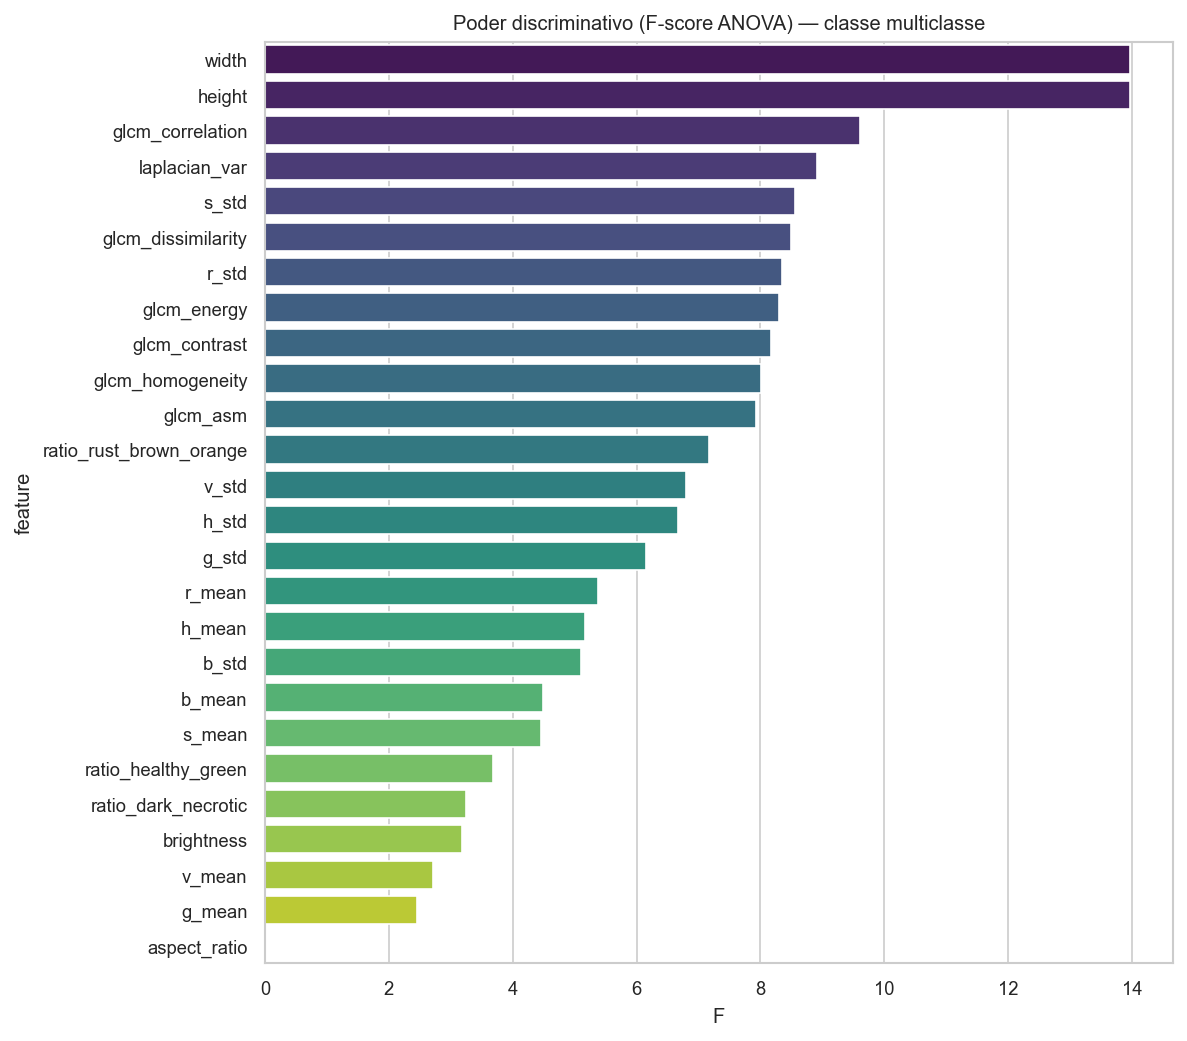
\includegraphics[width=\textwidth]{anova_fscore.png}

    \column{0.46\textwidth}
    \textbf{Achado contraintuitivo no F-\textit{score} (ANOVA):}
    \begin{itemize}
      \item \texttt{width} e \texttt{height} aparecem como \alert{features mais discriminativas} ($F=13{,}96$, $p<10^{-12}$)
      \item \texttt{ratio\_healthy\_green}: \textbf{maior} em \textit{rust\_level\_1} (0,743) do que em \textit{healthy} (0,714)
    \end{itemize}
    \vspace{0.4em}
    \begin{alertblock}{Interpretação}
      Diferentes classes foram fotografadas em \textbf{sessões distintas} $\to$ o modelo pode aprender ``atalhos'' de aquisição em vez de sintomas reais.
    \end{alertblock}
  \end{columns}
\end{frame}

% =============================================================
\begin{frame}{Insight 4 --- Redundância entre \textit{features}}
  \begin{columns}[c]
    \column{0.55\textwidth}
    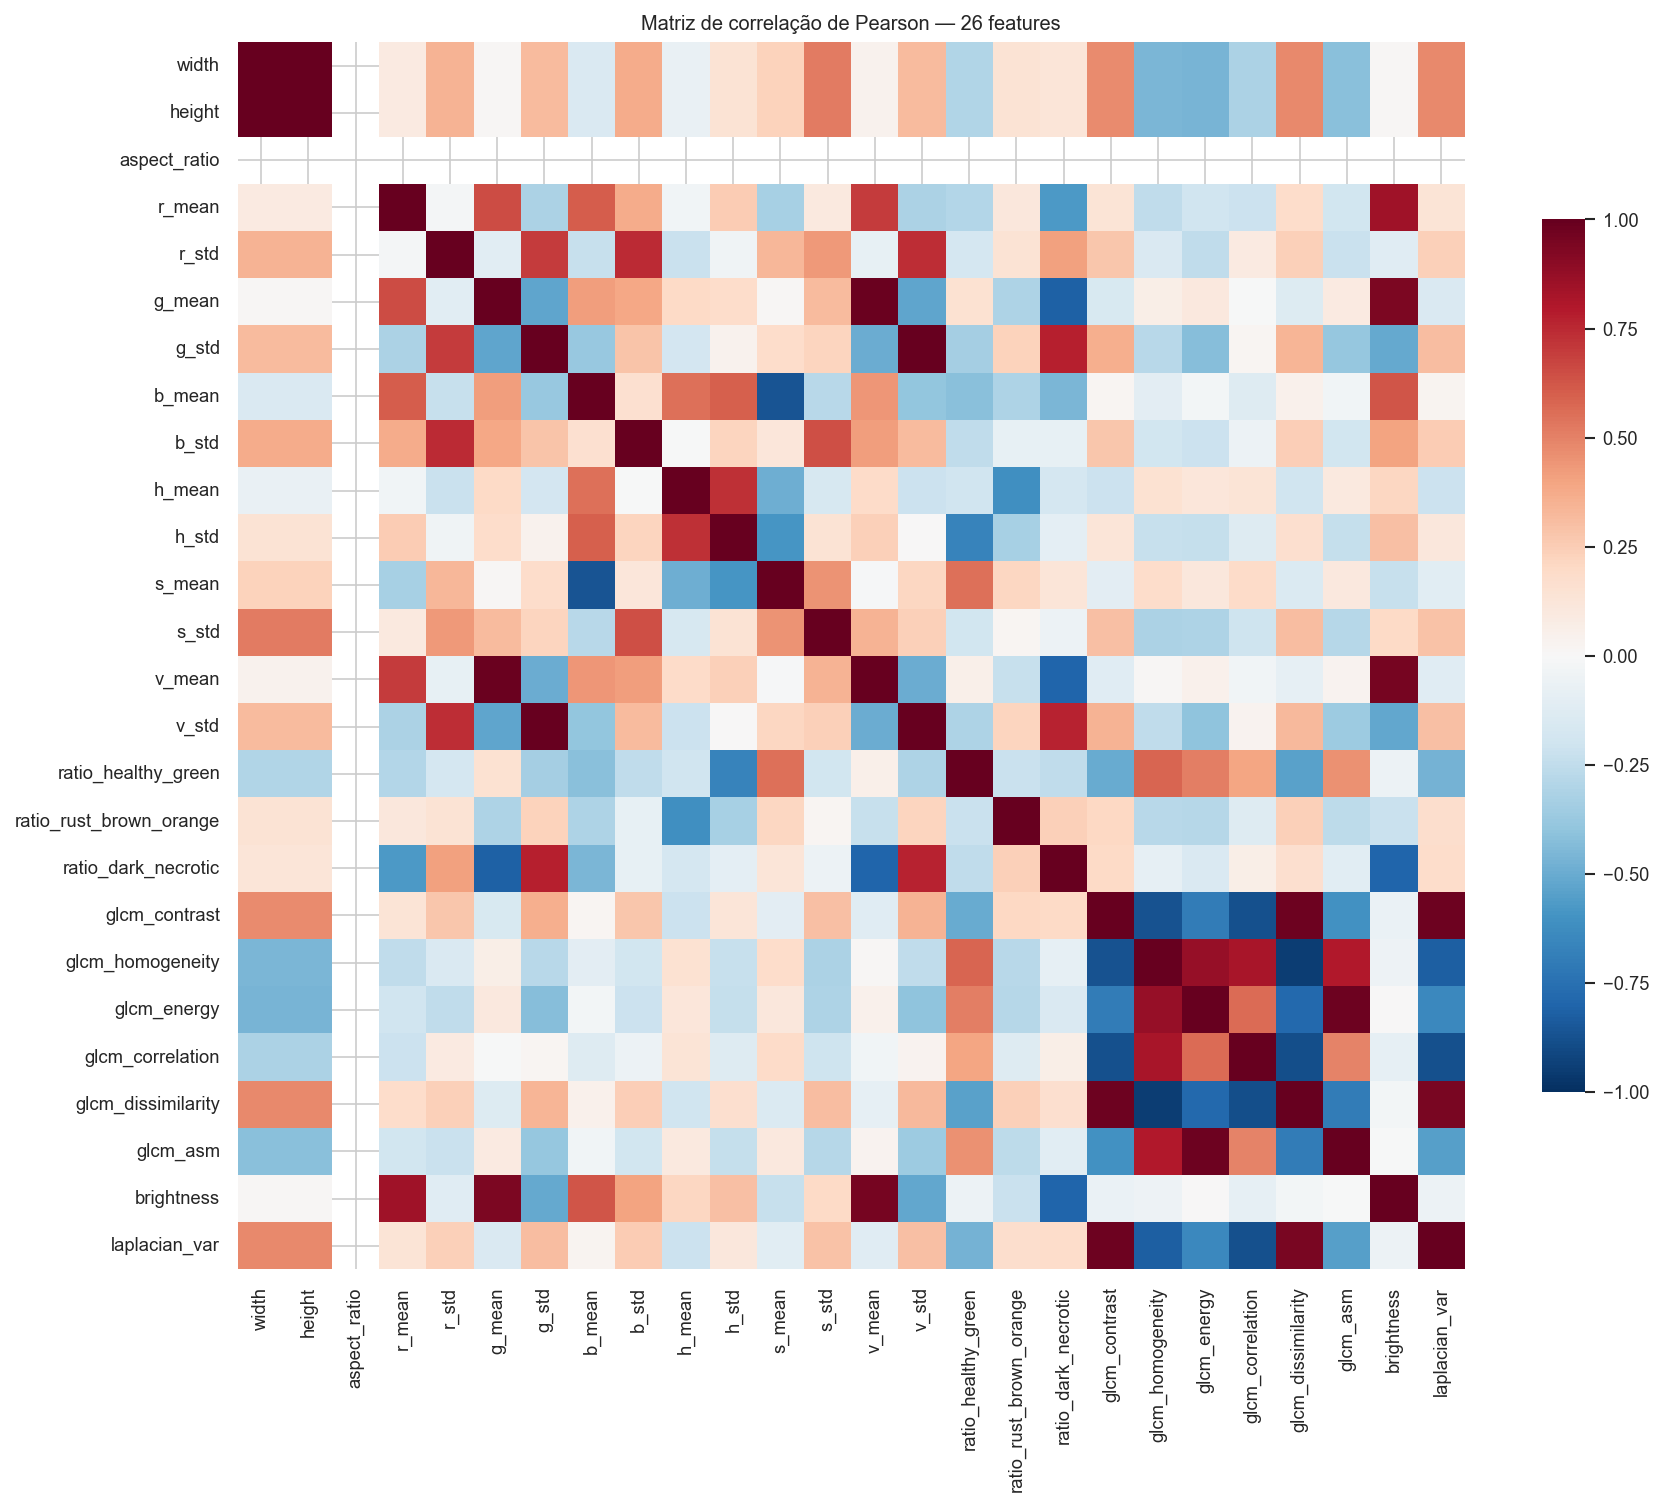
\includegraphics[width=\textwidth]{correlation_matrix.png}

    \column{0.45\textwidth}
    \small
    Top-5 pares mais correlacionados ($|r|$):
    \vspace{0.3em}
    \begin{tabular}{@{}llc@{}}
      \toprule
      A & B & $|r|$ \\
      \midrule
      \texttt{height} & \texttt{width} & 1{,}000 \\
      \texttt{g\_std} & \texttt{v\_std} & 0{,}994 \\
      \texttt{g\_mean} & \texttt{v\_mean} & 0{,}992 \\
      \texttt{glcm\_contrast} & \texttt{laplacian\_var} & 0{,}982 \\
      \texttt{glcm\_asm} & \texttt{glcm\_energy} & 0{,}981 \\
      \bottomrule
    \end{tabular}
    \vspace{0.5em}

    \normalsize
    Muitas dessas correlações são matematicamente esperadas (V = máx.\ de RGB; energia = $\sqrt{\text{ASM}}$).
  \end{columns}
\end{frame}

% =============================================================
\begin{frame}{Insight 5 --- Classes não separáveis linearmente}
  \begin{columns}[c]
    \column{0.62\textwidth}
    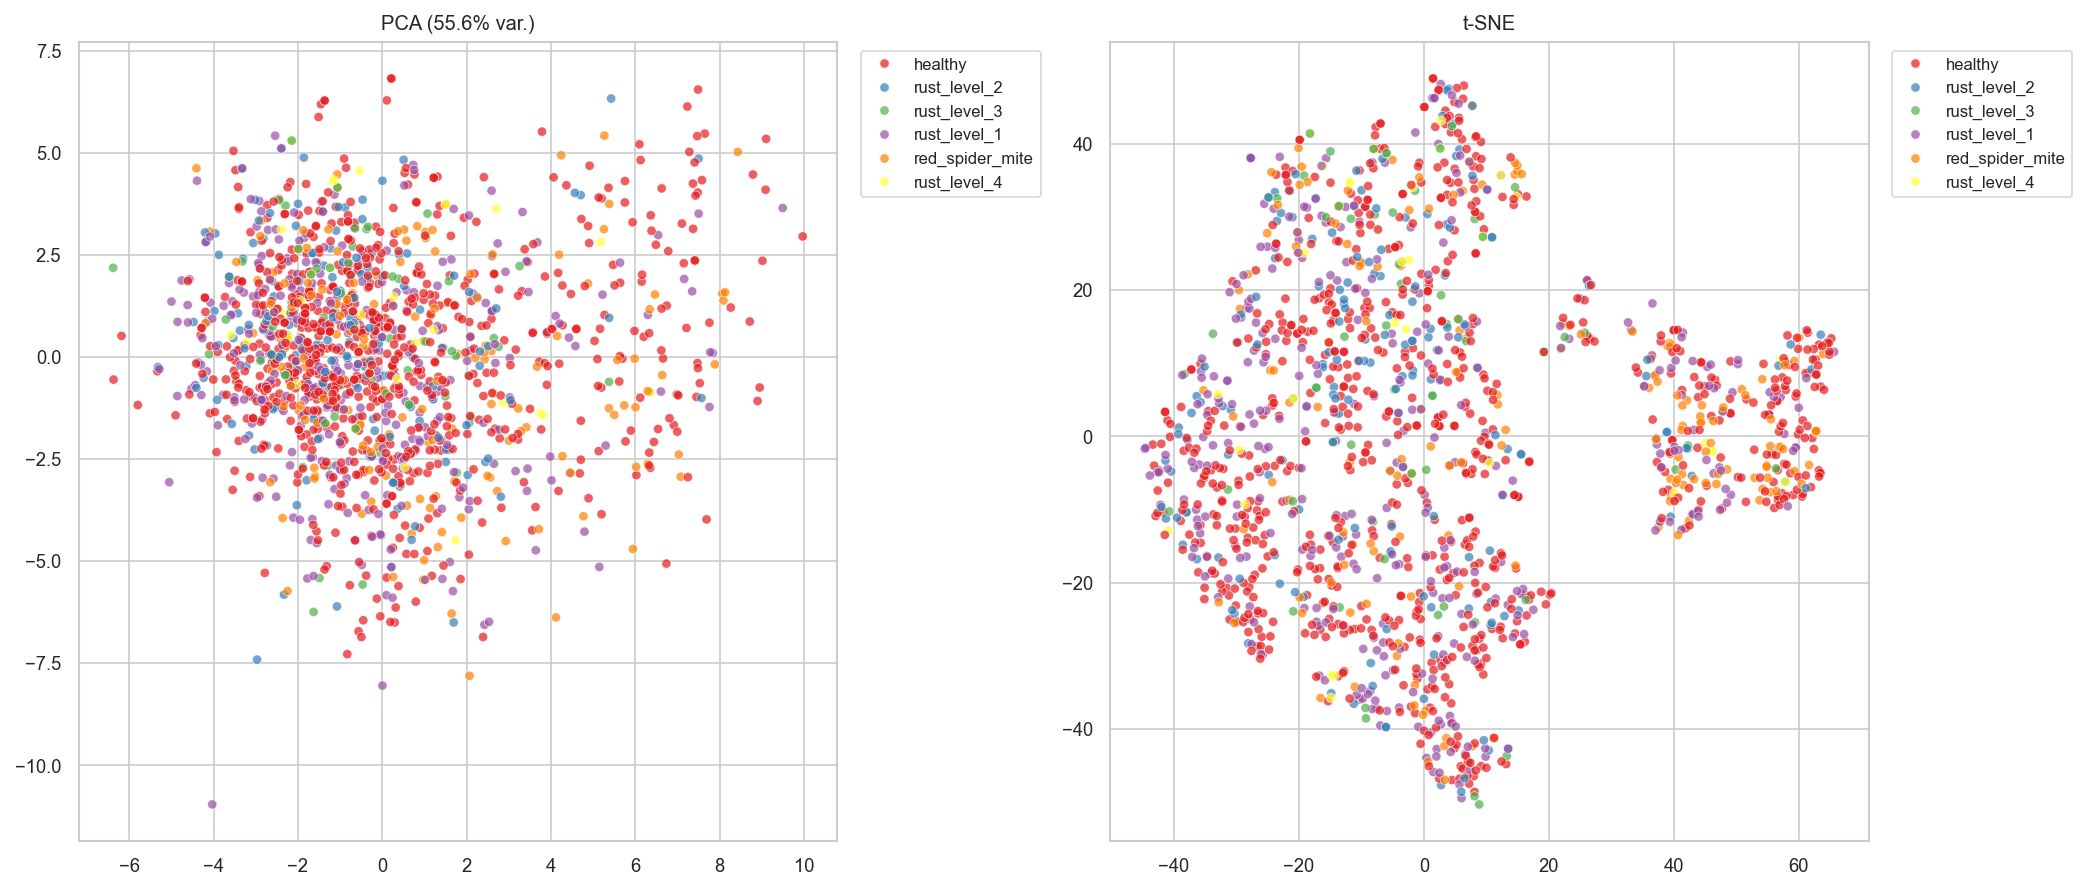
\includegraphics[width=\textwidth]{projections.png}

    \column{0.36\textwidth}
    \small
    \begin{itemize}
      \item \textbf{PCA:} sobreposição forte --- as duas primeiras componentes não separam as classes
      \item \textbf{t-SNE:} pequenos agrupamentos locais, mas sem separação clara global
      \item Expectativa: classificadores \textit{não lineares} (Random Forest, SVM-RBF) devem superar os lineares
    \end{itemize}
  \end{columns}
\end{frame}

% =============================================================
\begin{frame}{Dificuldades encontradas}
  \begin{itemize}
    \item \textbf{Anotações em múltiplos formatos}: CSV do Labelbox, JSON, COCO, VOC e XLSX. Escolhi o XLSX de classes por ser o mapeamento mais limpo arquivo$\to$rótulo.

    \vspace{0.3em}
    \item \textbf{Heterogeneidade de resolução}: imagens com até 8 MP exigiram redimensionamento antes do GLCM para manter o custo computacional tratável.

    \vspace{0.3em}
    \item \textbf{Decisão de representação}: converter imagens em \textit{features} tabulares foi uma escolha metodológica não trivial --- precisei desenhar \textit{features} que capturassem aspectos visualmente discriminativos (proporções cromáticas por HSV) e justificá-las.

    \vspace{0.3em}
    \item \textbf{Viés de aquisição não previsto}: o achado de que \texttt{width}/\texttt{height} são fortemente discriminativos foi inesperado e exige cuidado metodológico nas etapas subsequentes.
  \end{itemize}
\end{frame}

% =============================================================
\begin{frame}{Próximos passos --- Etapa 02}
  \begin{enumerate}
    \item Importar \texttt{rocole\_features.csv} no \textbf{KNIME}

    \vspace{0.3em}
    \item \textbf{Remover \textit{features} de dimensão} (\texttt{width}, \texttt{height}, \texttt{aspect\_ratio}) para mitigar o viés de aquisição identificado

    \vspace{0.3em}
    \item Particionamento estratificado 70\,\% / 15\,\% / 15\,\%

    \vspace{0.3em}
    \item Treinar e comparar classificadores clássicos: \textit{Decision Tree}, \textit{Random Forest}, \textit{Naïve Bayes}, SVM

    \vspace{0.3em}
    \item Avaliação com métricas sensíveis ao desbalanceamento: F1-\textit{macro}, \textit{balanced accuracy}, matriz de confusão

    \vspace{0.3em}
    \item Estabelecer \textbf{linha de base} quantitativa para posterior confronto com \textit{deep learning} na dissertação
  \end{enumerate}
\end{frame}

% =============================================================
\begin{frame}[allowframebreaks]{Referências}
  \footnotesize
  \begin{enumerate}
    \item PARRAGA-ALAVA, J.; CUSME, K.; LOOR, A.; SANTANDER, E. \textit{RoCoLe: A robusta coffee leaf images dataset}. Mendeley Data, v.2, 2019. DOI: 10.17632/c5yvn32dzg.2.

    \item SANTOS, L. F. C.; OLIVEIRA, G. M. B.; SILVA, R. R. V. Classificação de doenças em folhas de café robusta utilizando redes neurais convolucionais. In: SBC, \textit{Anais do Workshop de Computação Aplicada à Gestão do Meio Ambiente e Recursos Naturais}. Porto Alegre, 2023. p. 61--70.

    \item ESGARIO, J. G. M.; KROHLING, R. A.; VENTURA, J. A. Deep learning for classification and severity estimation of coffee leaf biotic stress. \textit{Computers and Electronics in Agriculture}, v. 169, p. 105162, 2020.

    \item MOHANTY, S. P.; HUGHES, D. P.; SALATHÉ, M. Using deep learning for image-based plant disease detection. \textit{Frontiers in Plant Science}, v. 7, p. 1419, 2016.

    \item BARBEDO, J. G. A. Factors influencing the use of deep learning for plant disease recognition. \textit{Biosystems Engineering}, v. 172, p. 84--91, 2018.

    \item BARBEDO, J. G. A. Plant disease identification from individual lesions and spots using deep learning. \textit{Biosystems Engineering}, v. 180, p. 96--107, 2019.

    \item HARALICK, R. M.; SHANMUGAM, K.; DINSTEIN, I. Textural features for image classification. \textit{IEEE Transactions on Systems, Man, and Cybernetics}, v. SMC-3, n. 6, p. 610--621, 1973.

    \item MATIELLO, J. B. et al. \textit{Cultura de café no Brasil: manual de recomendações}. 2. ed. Rio de Janeiro: MAPA/PROCAFÉ, 2016.

    \item Companhia Nacional de Abastecimento. \textit{Acompanhamento da safra brasileira de café}. 2024. Disponível em: \url{https://www.conab.gov.br}. Acesso em: jan.\ 2026.
  \end{enumerate}
\end{frame}

% =============================================================
\begin{frame}[plain]
  \vfill
  \centering
  {\Huge \color{cafeEscuro} \textbf{Obrigada!}}

  \vspace{1.2em}
  \large Dúvidas, sugestões e críticas são muito bem-vindas.
  \vspace{1.5em}

  \begin{tabular}{rl}
    \textbf{Natalia Salete Rodrigues} & \texttt{natsalete@ufu.br} \\
    PPGEELT / UFU & Mestrado em Engenharia Elétrica \\
  \end{tabular}
  \vfill
\end{frame}

\end{document}
